\documentclass{report}
\usepackage{graphicx} % Required for inserting images
\usepackage{float} % so that images are not at the end of the docuemnt
\usepackage[a4paper, top=20mm, bottom=20mm, left=25mm, right=25mm]{geometry}
\usepackage{subcaption}
\usepackage{titlesec}
\title{Visual Computing Assignment}


\author{Ebbe Wertz, Mathias Houwen}
\date{30 March 2025}

\begin{document}

\maketitle

\section{General similarity detection}
\label{sec:ssim}

Defects are detected by checking where similarity between the test and the template image is low. To do this, SSIM is used to produce a similarity map. Defects are recognized by a low similarity score. Therefore, a threshold is used to select regions of low similarity. The defects are indicated by finding the contours of each selected region. To avoid false detections from noise, only contours with a minimal area are accepted. Figure \ref{fig:ssim} shows a similarity map, with its result after applying the threshold.

\begin{figure}[H]
    \centering
    \begin{subfigure}[b]{0.45\linewidth}
        \centering
        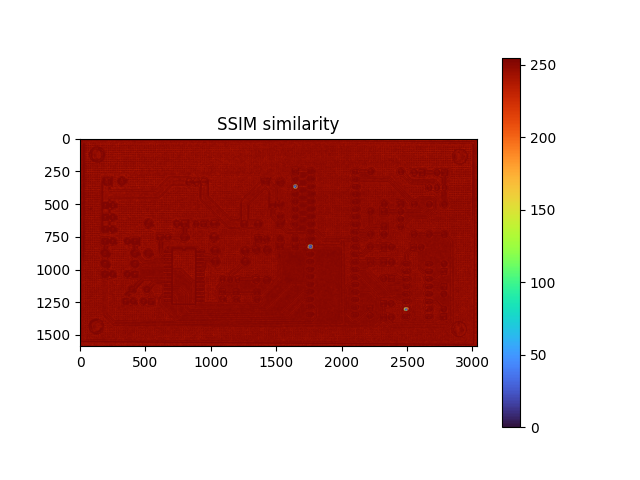
\includegraphics[height=50mm, keepaspectratio]{report_images/plots/ssim.png}
        \caption{SSIM similarity map}
    \end{subfigure}
    \hfill
    \begin{subfigure}[b]{0.45\linewidth}
        \centering
        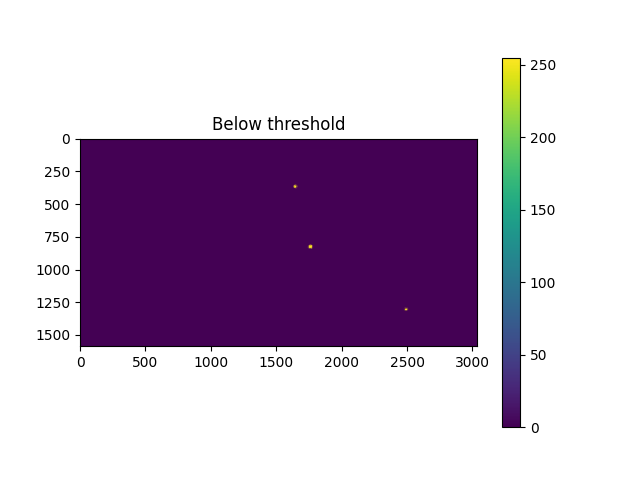
\includegraphics[height=50mm, keepaspectratio]{report_images/plots/thresh.png}
        \caption{Selected areas below threshold}
    \end{subfigure}
    \caption{Selected areas with threshold}
    \label{fig:ssim}
\end{figure}

In some cases, single defects are flagged as multiple, as seen in figure \ref{fig:BoxSlecht}. This is solved by merging all detection contours under a minimal distance. Figure \ref{fig:BoxGoed} shows the result.

\begin{figure}[H]
    \centering
    \begin{subfigure}[b]{0.45\linewidth}
        \centering
        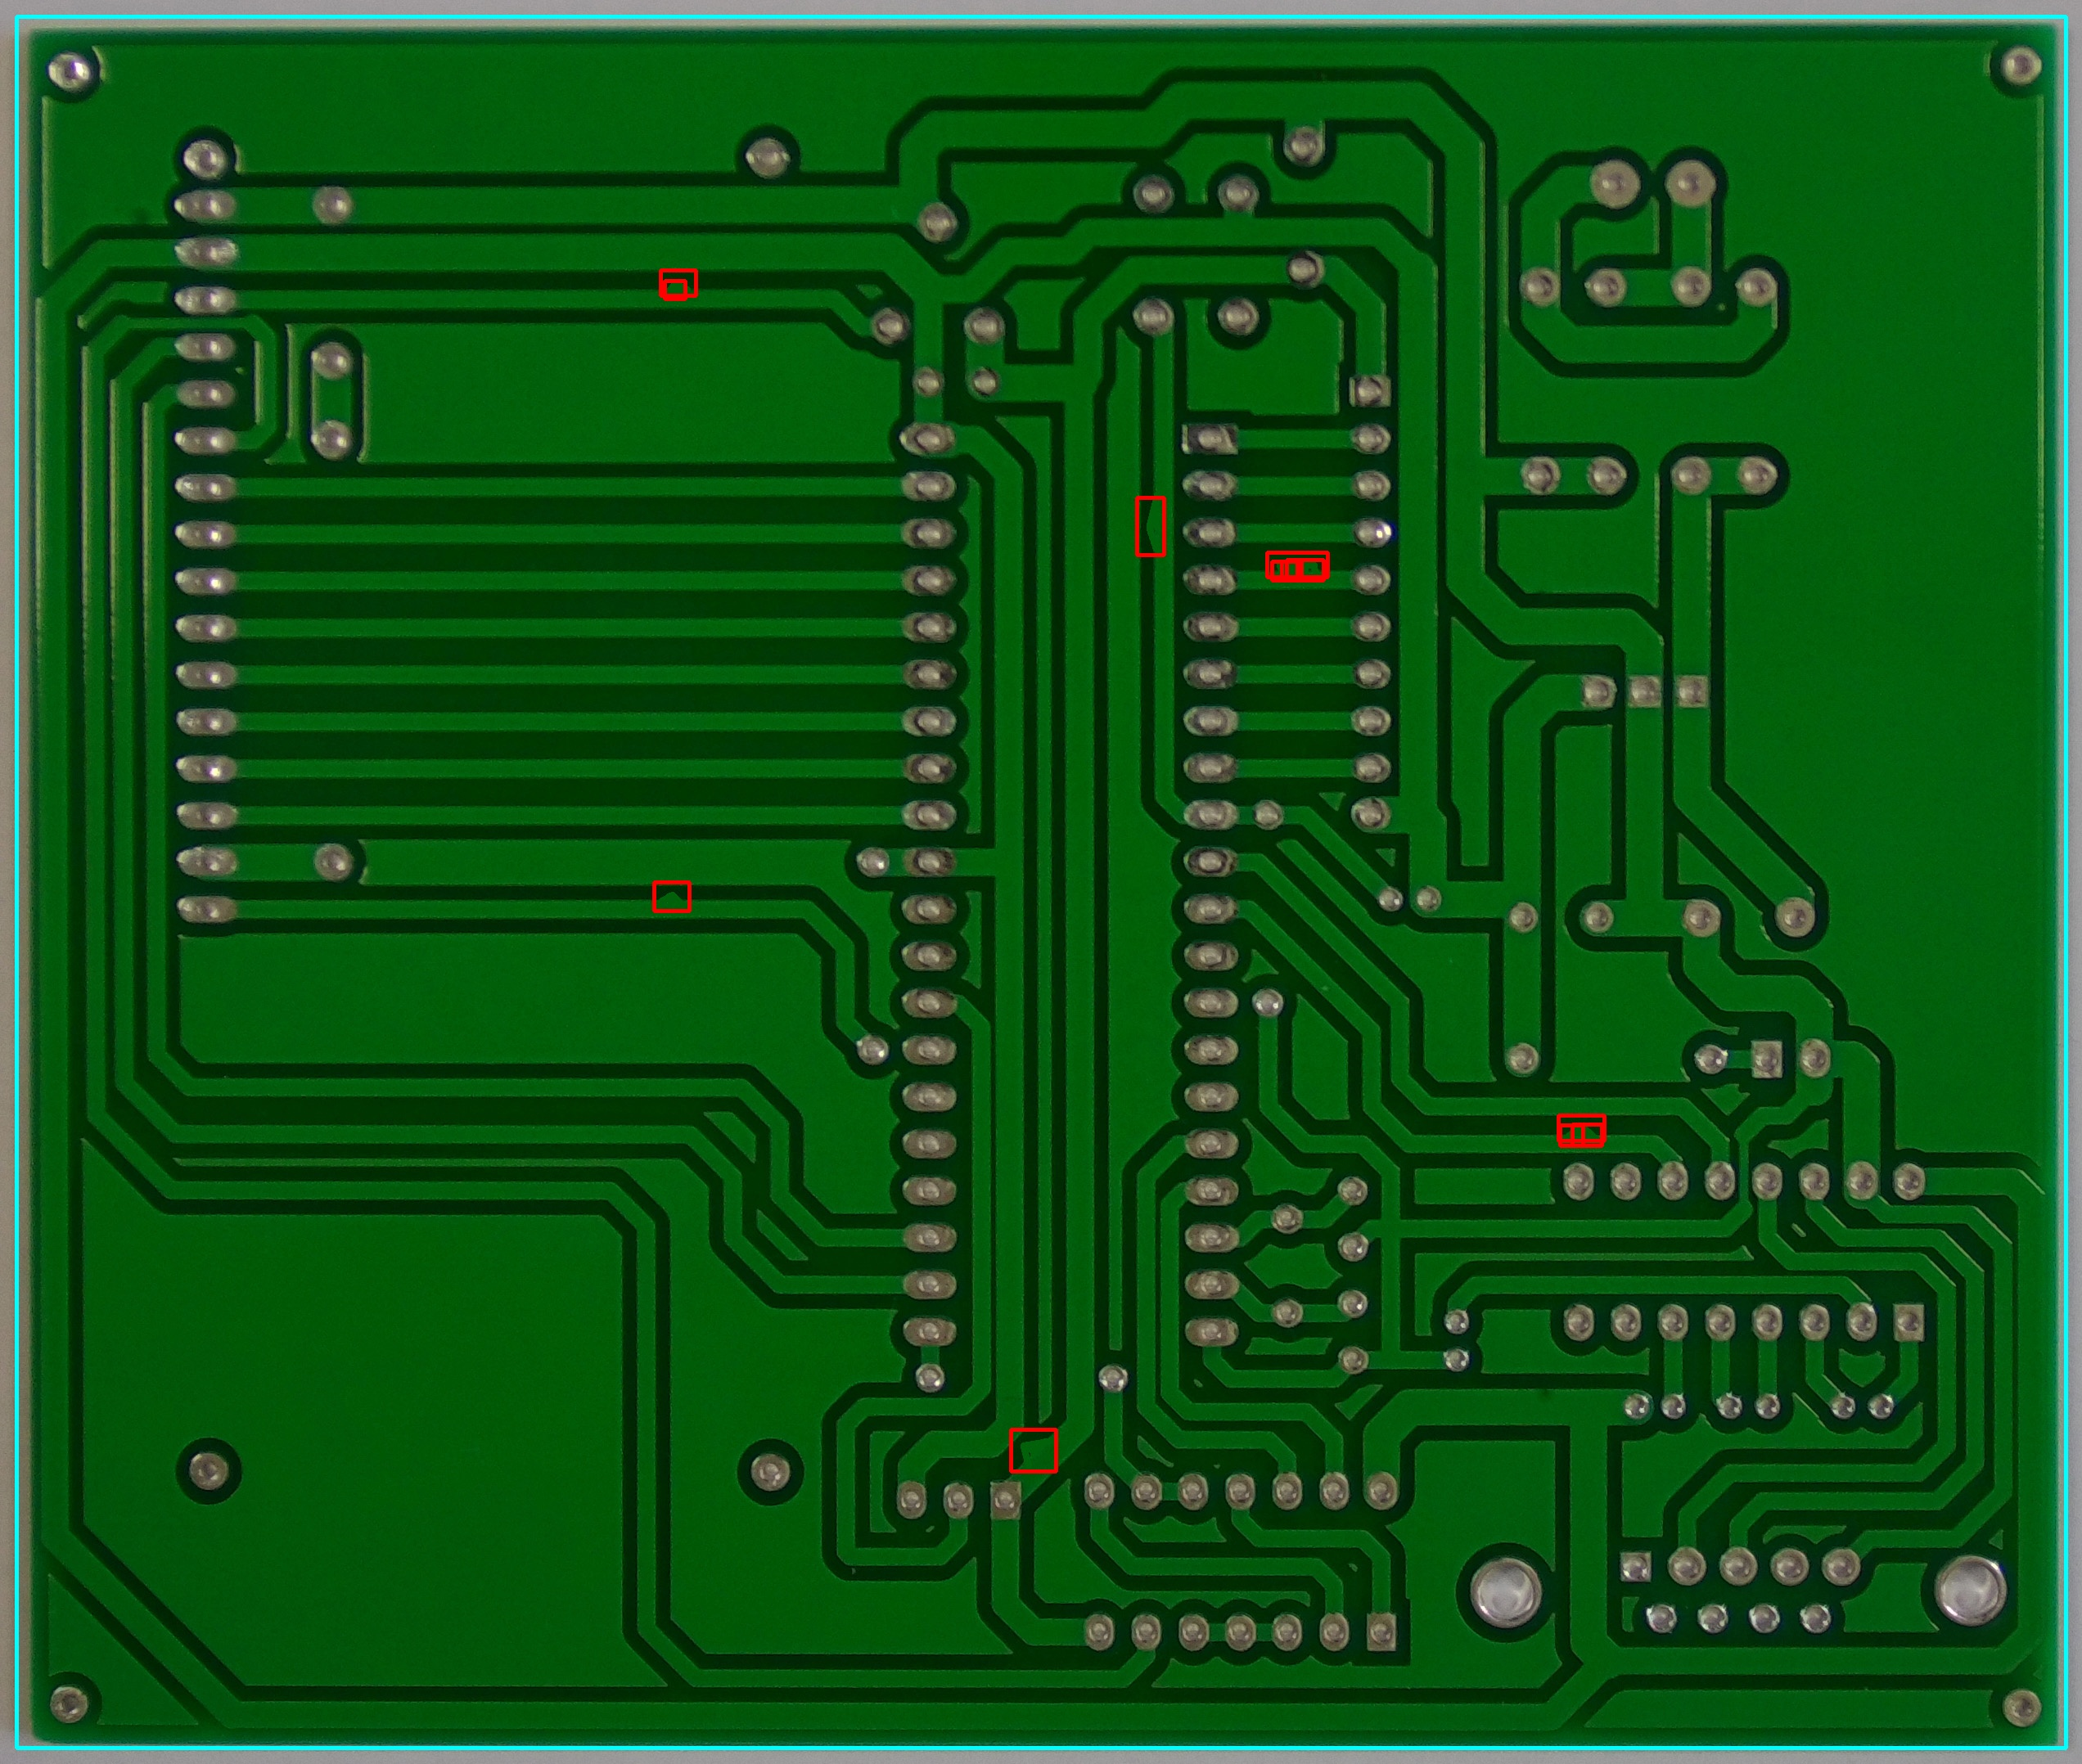
\includegraphics[height=50mm, keepaspectratio]{report_images/ouput_images/slecht zonder box merging.jpg}
        \caption{Overlapping defect indications}
        \label{fig:BoxSlecht}
    \end{subfigure}
    \hfill
    \begin{subfigure}[b]{0.45\linewidth}
        \centering
        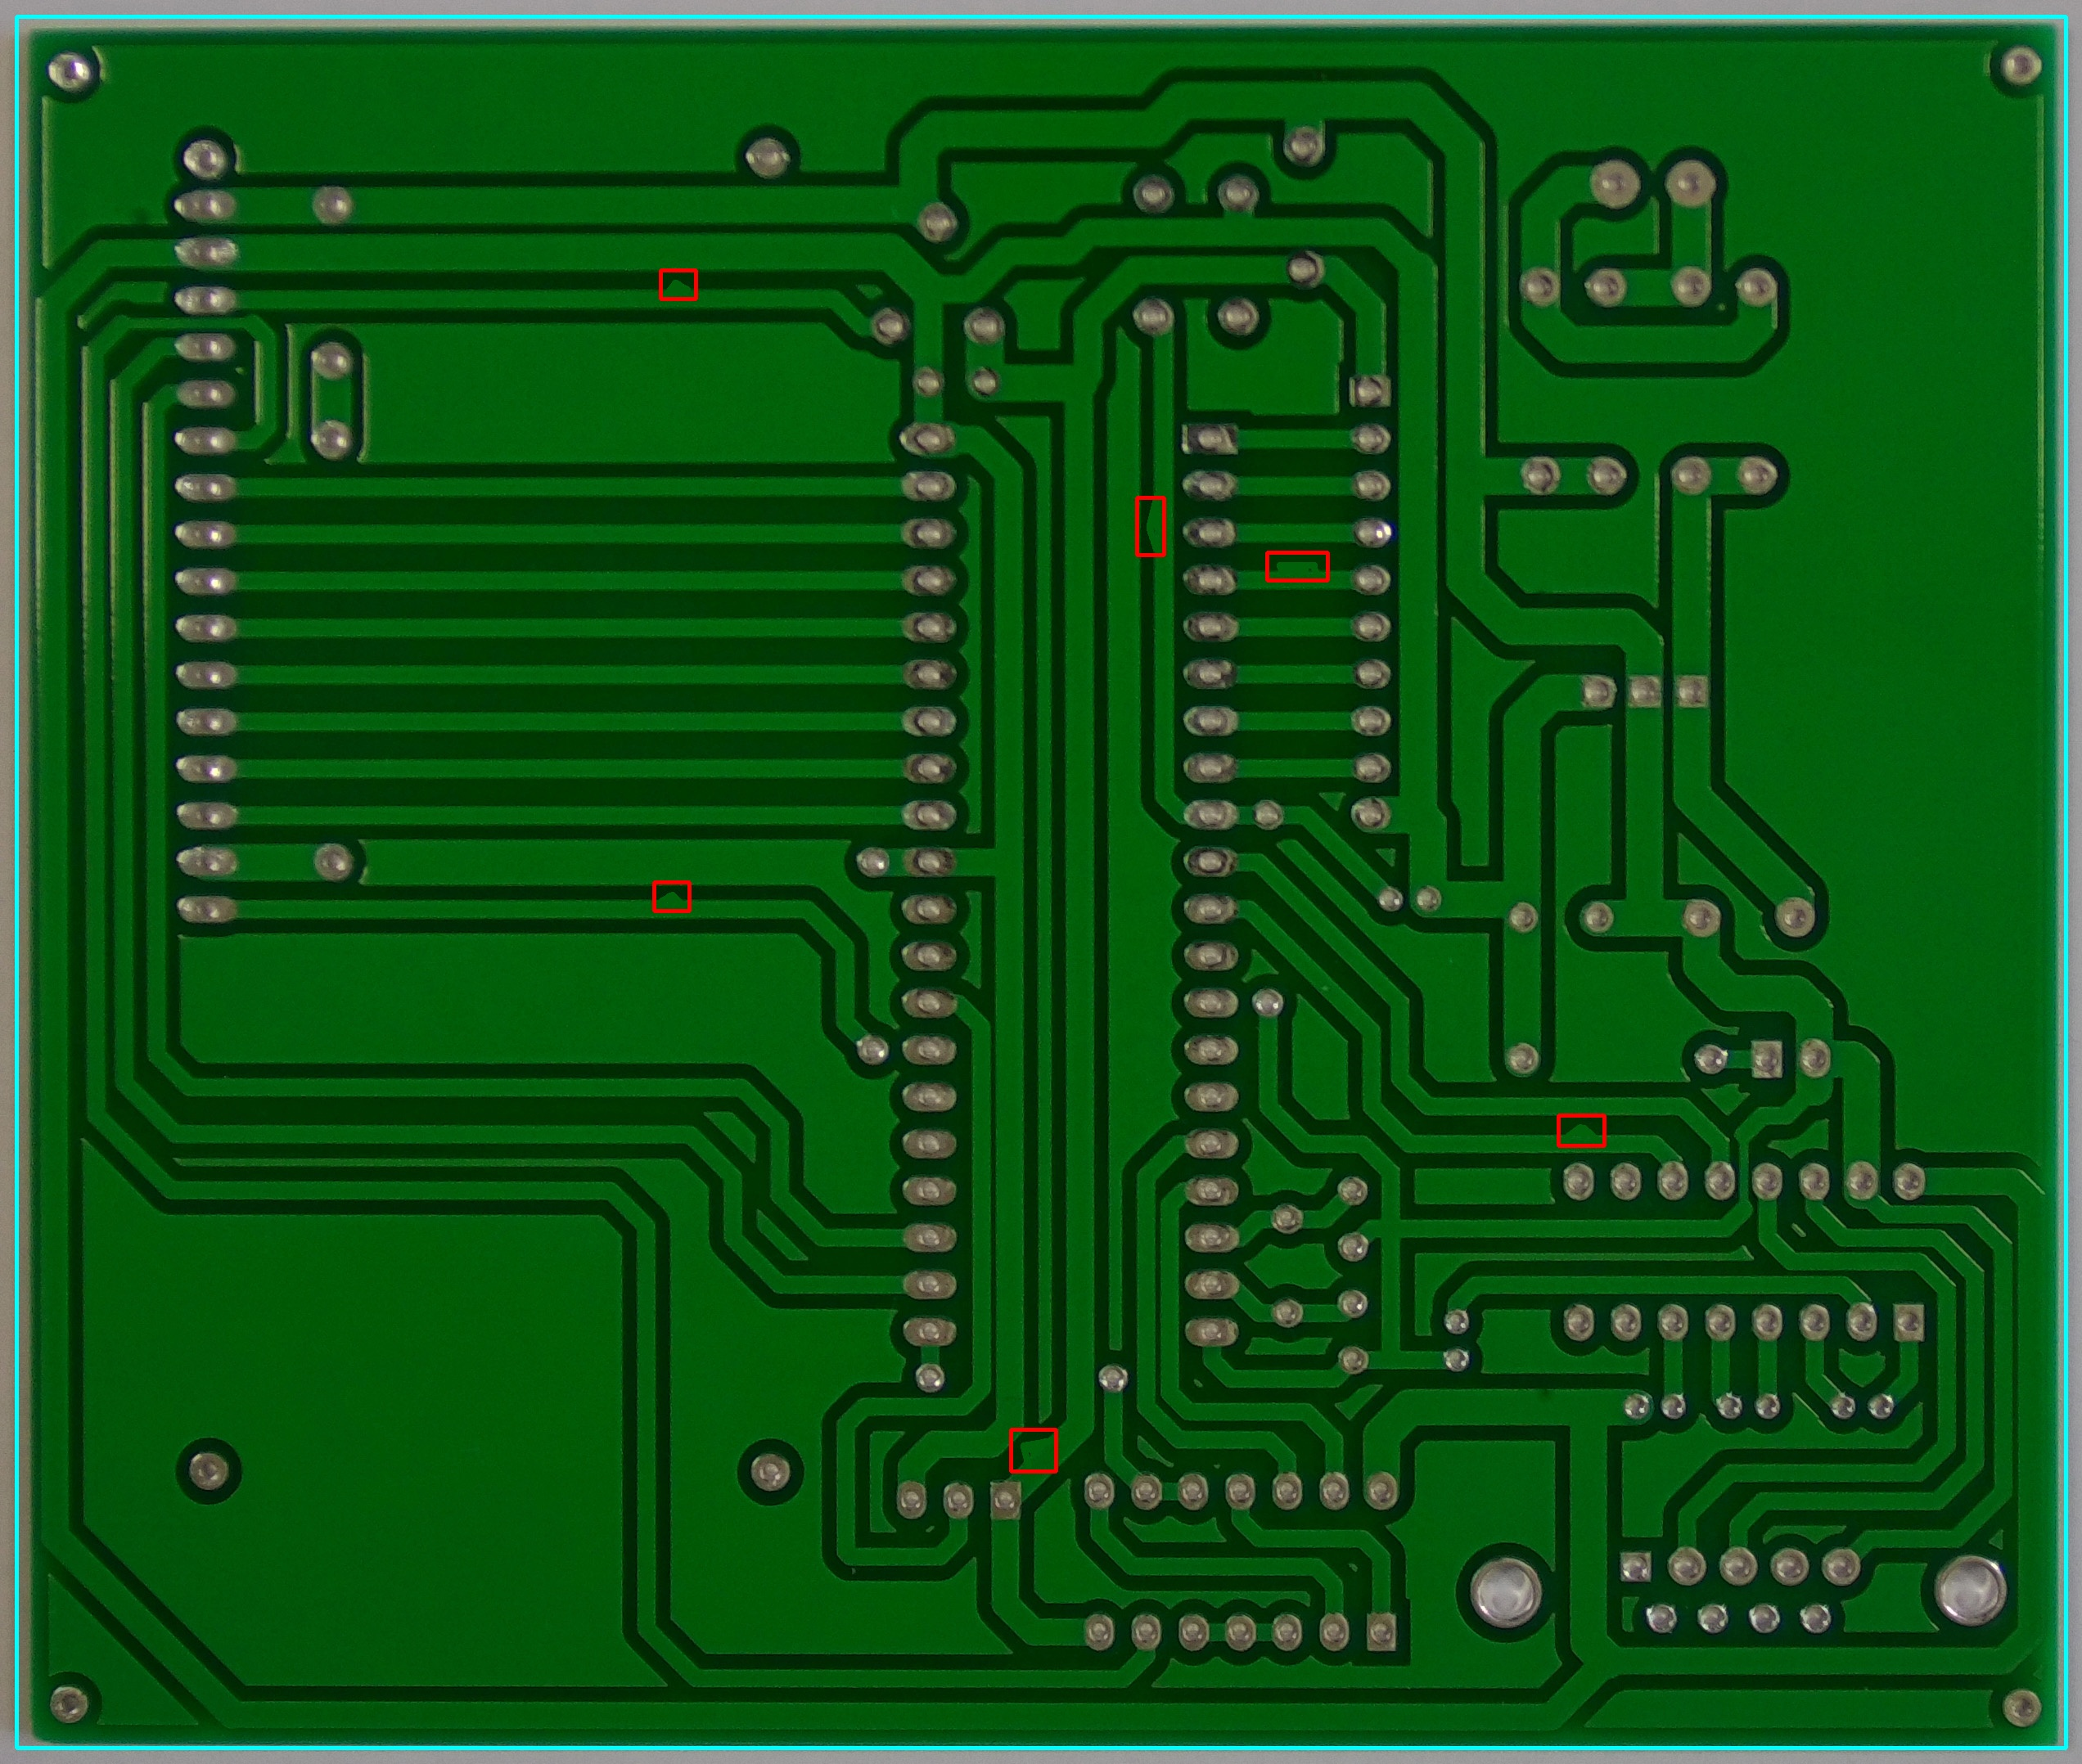
\includegraphics[height=50mm, keepaspectratio]{report_images/ouput_images/goed met box merging.jpg}
        \caption{Merged defects}
        \label{fig:BoxGoed}
    \end{subfigure}
    \caption{Defect detection using SSIM}
    \label{fig:DefectComparison}
\end{figure}

As a final precaution, the border of the image has a padding in which detection is ignored, as shown by the cyan box in both figures. This prevents detection of defects in the environment around the PCB, as well as artifacts that filters can introduce at the edge of an image.

\section{Handling noise}
\subsection{Uniform noise}

Noise primarily consists of high-frequency components, thus applying a low-pass filter is an effective approach.\\
To apply this to SSIM, both the template image and the test image are identically filtered before performing the SSIM detection.\\
\newline
For a smooth output with no artifacts, a Gaussian blur filter is used. For perfectly uniform noise, such as in the test\_2 samples, this is effective, since it averages the pixel values with a weighted kernel.\\

In contrast, salt-and-pepper noise, as in test\_3, can bias an average due to the extreme values of black or white pixels.
In this case, a median is a more accurate measure than an average, thus a median blur filter is used. Its kernel replaces its central pixel with the median value of its neighbors.

\subsection{Periodic noise}
% zeggen dat de periodic nature van de noise een zeer simpel defect is als je het in de fourrier transform (magnitude gedeelte) bekijkt. Dan kan een notch filter toegepast , overweging tss directe cirkel of gaussian notch
Periodic noise can be handled more effectively in the domain of the Fourier transform of the image, given the noise consists of a very specific frequency. In the Fourier domain this corresponds to very specific points with hight value. Therefore, an effective filter is to mask these points using a notch. For a smooth result, a gaussian notch is used. In figure \ref{fig:fourrier}, the noise is clearly identified by two mirrored star pairs, causing asymmetry. Figure \ref{fig:fourrier_notch} shows a notch filter applied.

\begin{figure}[H]
    \centering
    \begin{subfigure}[b]{0.45\linewidth}
        \centering
        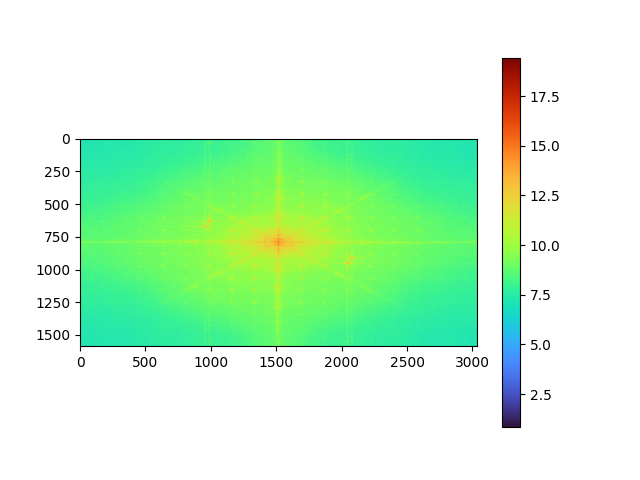
\includegraphics[height=50mm, keepaspectratio]{report_images/plots/fourrier.png}
        \caption{magnitude spectrum of Fourier transform}
        \label{fig:fourrier}
    \end{subfigure}
    \hfill
    \begin{subfigure}[b]{0.45\linewidth}
        \centering
        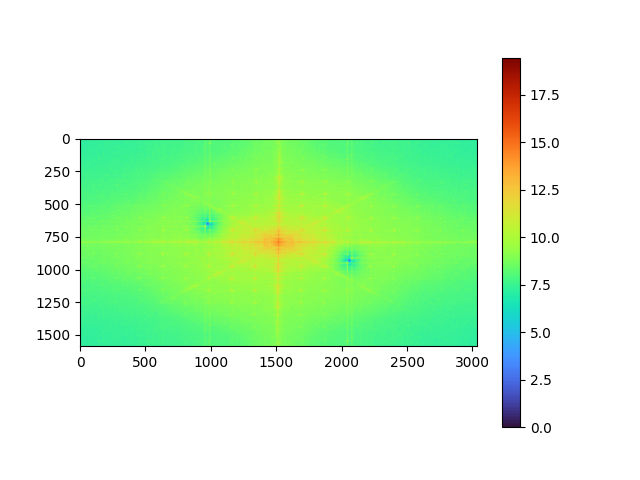
\includegraphics[height=50mm, keepaspectratio]{report_images/plots/fourrier_notch.png}
        \caption{Notch filter applied to spectrum}
        \label{fig:fourrier_notch}
    \end{subfigure}
    \caption{Removing noise using Fourier transform}
\end{figure}

\section{Handling transformations}

SSIM only operates on directly overlapped images, making transformed images unsuitable. Therefore the transformation must be inverted first. To detect the exact transformation, feature matching is used to relate the test and template images, after which a homography matrix is constructed from the matches to extract the exact transformation. SIFT is selected as the feature detector, and outputs keypoints and descriptors. A descriptor matching algorithm matches the corresponding keypoints. This approach is effective since feature matching is invariant to affine transformations.
Finally warping the image by the inverse homography matrix negates the transformation. However in practice, the template image is warped rather than the test image inversely warped, in order to keep SSIM in the perspective of the test images. Figure \ref{fig:match} shows the matched features. Figure \ref{fig:homo_ssim} shows SSIM applied on the transformed template image. Notice that the blank corner triangles resulting from rotation are masked by a value of 255. Erosion is also used to thicken the edges of this mask, to prevent the edge of the original template image to cause a low SSIM score.

\begin{figure}[H]
    \centering
    \begin{subfigure}[b]{0.45\linewidth}
        \centering
        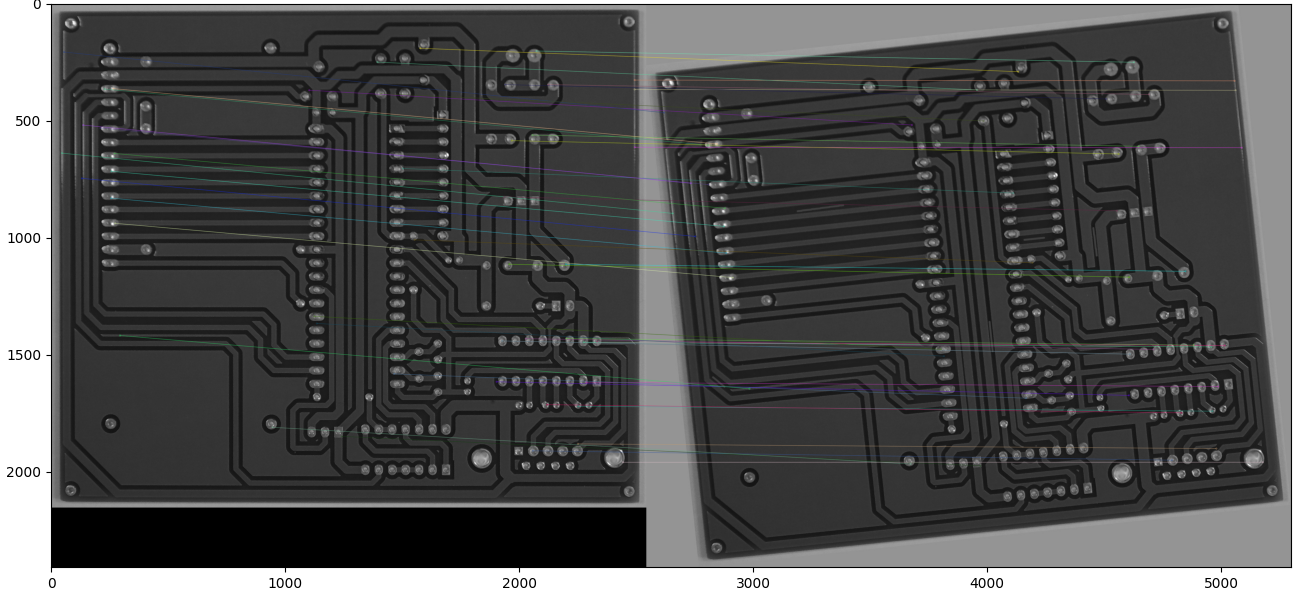
\includegraphics[height=40mm, keepaspectratio]{report_images/plots/match.png}
        \caption{Matched features by SIFT}
        \label{fig:match}
    \end{subfigure}
    \hfill
    \begin{subfigure}[b]{0.45\linewidth}
        \centering
        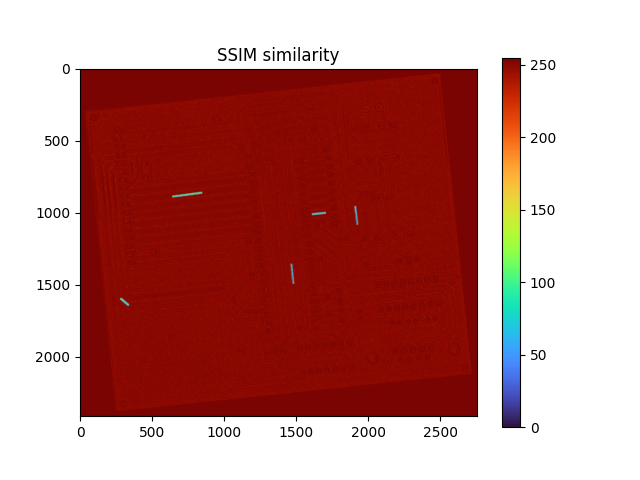
\includegraphics[height=50mm, keepaspectratio]{report_images/plots/homo_ssim.png}
        \caption{SSIM with template warped by homography}
        \label{fig:homo_ssim}
    \end{subfigure}
    \caption{SSIM with feature matching}
\end{figure}

\end{document}
